
\documentclass[10pt,onecolumn]{article}

\usepackage{graphicx}
\usepackage{wrapfig}
\usepackage{todonotes}
\usepackage{amssymb}
\usepackage{subfig}
\usepackage{booktabs}
\usepackage{url}
\usepackage{todonotes}
\usepackage{graphicx}
\usepackage{amsthm}
\usepackage{array}
\usepackage{enumitem}
\usepackage{adjustbox}
\usepackage{xcolor}
\usepackage{soul}
\usepackage[sort, numbers]{natbib}


\title{Statement for Mid-Probationary Review \\
Neil Klingensmith}
\date{}



\textwidth=7.5in
\textheight=9.25in
\columnwidth=3.33in
\columnsep 0.33in  %Space between columns
\hoffset=-0.5in \voffset=-0.125in \oddsidemargin=0in \topmargin=0in
\headheight=0in \headsep=0in



\newcolumntype{R}[2]{%
    >{\adjustbox{angle=#1,lap=\width-(#2)}\bgroup}%
    l%
    <{\egroup}%
}
\newcolumntype{C}[1]{>{\centering\arraybackslash}p{#1}}
\newcommand*\rot{\multicolumn{1}{R{25}{1em}}}% no optional argument here, please!


\begin{document}

\maketitle
\iffalse
\begin{wrapfigure}{tr}{5in}
\centering
     \captionsetup[subfigure]{justification=centering}
     \begin{subfigure}[b]{0.3\textwidth}
         \centering
         \includegraphics[width=\textwidth]{figures/vkey-powerstrip.png}
         \caption{A \textsc{VoltKey} charging a phone.}
         \label{fig:powerstrip}
     \end{subfigure}
     \begin{subfigure}[b]{0.3\textwidth}
         \centering
         \includegraphics[width=\textwidth]{figures/voltkey.png}
         \caption{Components of the \textsc{VoltKey} USB charger.}
         \label{fig:voltkey}
     \end{subfigure}
     \caption{The \textsc{VoltKey} platform.}
\end{wrapfigure}
\fi


\section{Overview}

In this statement, I outline my accomplishments in research, teaching and service since my arrival at Loyola in August 2019.

\section{Research}

My work aims to build platforms for a secure and efficient internet of things.
Since joining the faculty at Loyola, I have published seven peer-reviewed papers and been awarded two externally-funded grants totalling \$750,000.

Overall, the quality of my work is on the same level as many big-name R1 research labs.
My students are presenting at conferences alongside other top mobile and IoT researchers.
The conferences where our work is presented: IPSN~\cite{moonshine}, HotMobile~\cite{v2vposter,ucbitgenposter}, Ubicomp~\cite{voltkey,aerokey}, PoPETS~\cite{mutebutton}, and others, are all highly-competitive top-tier conferences.
And the work that my group submits to these conferences is all student-led.



\subsection{External Funding}

\begin{enumerate}
\item 

    {\bf Taming Container Privileges using Userland OS Guests}, \\
    PI, \$500,000, NSA January 2023 - December 2024 

\item
    {\bf Collaborative Research: OAC Core: Advancing Low-Power Computer Vision at the Edge}, \\
    Co-PI, \$250,000, NSF Award Number 2107020 July 2021 - July 2024 
	
\end{enumerate}

\subsection{Ongoing Research Projects}

My group is working in three active research areas, each focused on a different aspect of security and efficiency of the IoT.

\subsubsection{Securing Containers}


%The privilege model for containers is broken.
Linux containers---colloquially a lightweight alternative to virtualization---share a kernel and many resources with the host, e.g. memory, files, and users and groups.
But they are subject to container escapes, in which a process inside of the container can gain root privileges in the host.
Although sharing resources can provide a low-overhead execution environment for guest processes, it has the undesirable side-effect of blurring the boundaries between host and guest.
While workarounds exist to separate privileges and resources between container and host---\texttt{cgroups} and process namespaces---they do not perfectly isolate the runtime environment of the container.
Guest processes inside a container share users and groups with their associated privileges with the host.
Launching a new container requires issuing a complex sequence of privileged system calls to the host, each of which may break the isolation of the guest if done incorrectly.
Without isolation, untrusted containers can escape their process jails and modify the state of the host.


\begin{figure}[tb]
    \centering
  \subfloat[Conventional virtualization]{%
        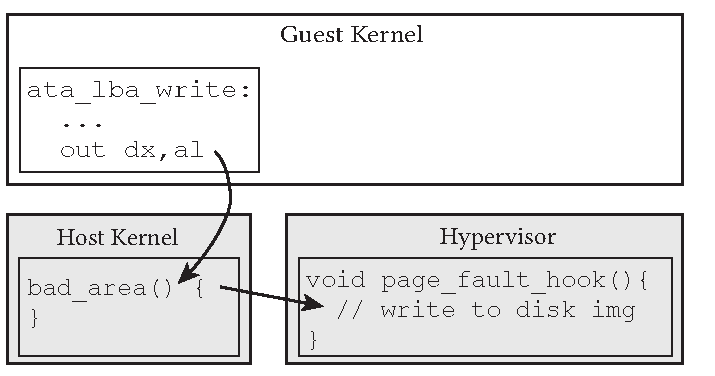
\includegraphics[height=4.5cm]{figures/conventional-diagram.pdf}\label{fig:conventional-diagram}}
  \subfloat[Userland virtualization]{%
      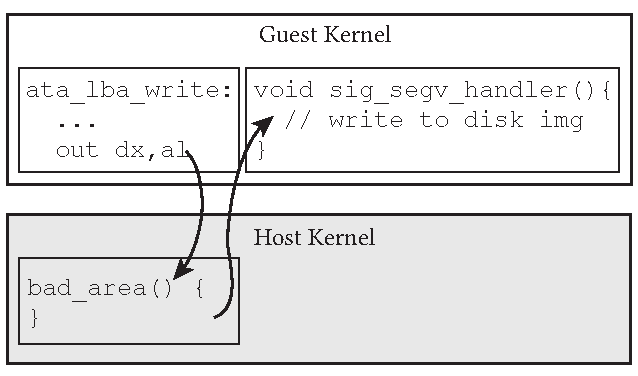
\includegraphics[height=4.5cm]{figures/uservirt-diagram.pdf}\label{fig:uservirt-diagram}}
  \caption{Privileged operation emulation in conventional and user mode containerization. Shaded modules execute in supervisor mode.}
  \label{fig:diagram}
\end{figure}


In this project, we are  developing a new execution environment to isolate untrusted containers from their host(s).
Untrusted containers can cause damage to the host system by escaping and modifying the state of the host system.
Container escapes are possible because of weak resource and privilege isolation between host and container.
The motivating idea behind the proposed work is to build a configurable containerization environment with stronger separation between container and host.
The key to improving isolation is allowing containers to be installed and managed by \emph{unprivileged users} on the host system with no need for elevated privileges to launch new container instances.
We call this technique \emph{userland containerization}.
Our approach will be to run the containers's software inside a sandboxed user mode Linux instance that---unlike conventional containers---strongly isolates privileges and other system resources from its host.%can transparently capture, filter, and anonymize data before higher level software gains access to it, giving users control of the overall data filtering policy.


\subsubsection{Computer Vision on the Edge}


Computer Vision (CV) on the Edge offers tremendous societal benefits, from finding missing persons to fighting forest fires.
These benefits can be realized through widespread deployment of cheap, low-power cameras and embedded chips.
However, these applications of CV have tight performance and time constraints, while current CV techniques assume powerful machines in the high-latency Cloud.
We propose holistic improvements to bring about the next generation of low-power, low-latency CV at the Edge.

Many innovations are needed to adapt the current generation of CV techniques to the Edge.
The current generation of CV is successful at many CV tasks, including classification, object detection, and facial recognition.
However, most CV efforts target general-purpose computing contexts, e.g., powerful mobile devices with access to the Cloud.
This resource-rich context permits state-of-the-art CV to use complex deep neural networks (DNNs) trained on high-quality images.
Unfortunately, many of these assumptions fail at the Edge.
Existing datasets do not suit the low-quality images available at the Edge.
Existing DNN model architectures are too complex for the resource constraints of Edge-class devices.
Existing engineering practices result in costly errors (energy, compute time) as we optimize architectures for the Edge.
And once suitable models are trained, many CV applications require new low-power distributed computing techniques.



\subsubsection{Zero Involvement Pairing and Authentication (ZIPA)}

\begin{wrapfigure}{tr}{3in}
\centering
\includegraphics[width=2.9in]{figures/voltkey.png}
\caption{The \textsc{VoltKey} USB charger.}
\label{fig:voltkey}
\end{wrapfigure}

Context-based zero-involvement authentication and pairing (ZIA and ZIP) is a set of techniques that allow nearby devices to form self-organizing networks using authentication tokens derived from ambient environmental noise like electromagnetic radiation, audio, vibrations, etc.
Random number generators commonly use ambient environmental noise collected from the timing of I/O events as a source of entropy.
ZIA and ZIP techniques build on that idea to use correlated environmental noise to construct shared authentication and pairing tokens.
Environmental noise encodes entropy that can be simultaneously measured by a group of nearby devices which extract identical authentication or encryption tokens.
Measurement of the same environmental noise signals is evidence that each device in the group is located in the same physical location at the same time and should belong to the same user.


\textsc{VoltKey}, a ZIA platform developed in my lab (prototype shown in Figure \ref{fig:voltkey}), uses shared random voltage fluctuations on a building's electric power lines to automagically generate a shared private key.
Two devices drawing power through \textsc{VoltKey} USB chargers in the same building can join the same encrypted WiFi network using a common key generated by the \textsc{VoltKey} devices without a user entering a password.
Figure \ref{fig:pipeline} showcases the process of key generation.
To generate a ZIA key, algorithms commonly share three steps:

\begin{figure}
\includegraphics[width=\hsize]{figures/datapipeline.pdf}
\caption{Data pipeline used to establish a key from ambient environmental randomness in Zero Involvement Authentication.}
\label{fig:pipeline}
\end{figure}


\begin{enumerate}%[leftmargin=0cm,itemindent=.5cm,labelwidth=\itemindent,labelsep=0cm,align=left]
    \item \textbf{Noise Harvesting:} In the first step, the device gathers a sequence of samples from an environmental noise process.
    This is usually done by a microcontroller with an analog-to-digital converter.
    These samples are typically filtered to remove undesirable features and time synchronized by sending messages over a public channel.
    \item \textbf{Bit Extraction:} Raw samples gathered from the environmental noise process are then converted by a fuzzy extractor into a sequence of bits that will be a key.
    Generally, a few bit errors (1-10\%) between authenticating devices are permitted in the extracted bit sequence.
    The most popular bit extraction technique is to divide the sequence of raw noise samples into bins of 10-20 samples each and compute a function on each bin that generates a $1$ or a $0$.
    \item \textbf{Key Reconciliation:} After bit extraction, each device will have a sequence of bits in memory that represents a key.
    Even though the devices are located nearby one another, differences in their measurements of the raw environmental noise will have caused spurious errors in the extracted bit sequences.
    Key reconciliation is the process by which two nearby devices exchange messages with one another over a public channel to resolve those bit differences.
    At the end of this step, if both devices are honest and located in the same vicinity, they will each hold identical authentication keys that can be used to encrypt data or validate their identities to one another.
\end{enumerate}


Physical location is a good proxy for identity because we already have well-established and enforceable methods for restricting physical access to private spaces.
For instance, we occasionally and selectively admit people into our personal homes, and devices inside our homes can be assumed to have gone through some amount of authentication before entering.
Such identity attestation can be used in a variety of practical scenarios.
My ongoing work is focused on building techniques for ZIA and ZIP systems for use in consumer, industrial, and military networks.

\begin{wrapfigure}{tr}{4in}
\centering
\includegraphics[width=3.75in]{figures/introduction.pdf}
\caption{System and threat models of \textsc{VoltKey}. A number of IoT devices are installed in each home. WiFi range of each home can reach neighboring homes, potentially the adversary's.}
\label{fig:introduction}
\end{wrapfigure}


\paragraph{Universally Composable Key Establishment}

In order to be practical, Zero-Involvement key generation should be universally-composable and must consistently generate high-quality keys, regardless of environmental conditions.
Existing ZIA and ZIP systems do not provide universally composable security, which among other consequences, means that only a pair of devices can agree on a common key.
Large networks that share a single key are not possible.
%In our early work to evaluate key quality of ZIA and ZIP systems~\cite{moonshine}, we found a lot of variability in the randomness of the keys generated by the systems we studied.


Many ZIA and ZIP key generation schemes generate correlated bit sequences from time series measurements of an environmental noise source.
Generally, a sequence of digitized samples is divided into blocks, and bits are chosen by computing a function on each block of samples\cite{voltkey,Lin-H2B,Lee-WiSec20}.
This approach tends to be very sensitive to small shifts between the buffers of digitized samples gathered from the environmental noise, usually requiring the buffers to be aligned to the granularity of a single sample.
Sample buffer alignment is usually achieved by one device sharing a portion of its samples with all other devices in the network which in turn align their sample buffers to match.


The process of one device sharing a portion of its sample buffer with the other nodes in the network breaks the assumptions of universally composable security.
By sharing a substantial portion of its measurements of the environmental noise signal, a legitimate node divulges information that could be used by an illegitimate eavesdropper to refine her guess about the key that the exchange will ultimately generate.
Consequently, there is no guarantee that these ZIA and ZIP techniques can be generalized to networks of an arbitrarily large number of nodes.
Indeed, all of the testbeds of ZIA and ZIP systems we are familiar with create unique authentication tokens for each node that joins a network.
%The intuition is that this sample buffer alignment shares a non-negligible amount of information about the underlying environmental noise signal with eavesdroppers


To make ZIA and ZIP schemes universally composable, we will introduce a modification to standard bit extraction techniques that allows their key agreement protocol to conform to the assumptions of UC security.
Our modification simply relaxes the requirement that the buffers containing the digitized samples of environmental noise be aligned down to to a single sample.
The result is that there is no need for one device in the network to share a portion of its sample buffer with the rest of the nodes.
Because there is no need to share a subset of the environmental noise sample buffer, the key establishment protocol leaks no information about 

Our approach is to generate bits for the authentication token from the frequency spectrum of the environmental noise signal, which has the desirable property of being time shift-resistant (as long as the time shifts are relatively small).
Previous attempts to make use of the frequency domain representation of an environmental noise signal have not been successful because most of the harmonics in the frequency spectrum are not shared among authenticators.
Our approach is to use a version of principal component analysis (PCA), which selects a linear combination of the dominant harmonics in the environmental noise signal as the basis for generating a key.
In many settings, the dominant harmonics are common to all of the authenticators that share similar versions of the environmental noise signal.
Our approach uses a warmup period during which authenticators continuously sample the environmental noise, generate a covariance matrix from the noise signal, and finally perform an eigenvector decomposition on the covariance matrix to find the dominant signal components.
We then project samples of the environmental noise into the subspace spanned by the dominant eigenvectors of the covariance matrix to generate a key.

A major challenge of relying on PCA for key generation is porting the software to resource-constrained embedded platforms, most of which cannot even hold the covariance matrix in memory.
We have developed a relaxation of PCA which can find an approximate solution without constructing the covariance matrix and computing its eigenvector decomposition.




\paragraph{Key Quality in ZIA Systems}



Most environmental noise sources generate signals with a low \emph{randomness density}.
Informally, we say that if we harvest a $k$-bit key from an environmental source, that key could be represented with a shorter sequence of $k-n$ bits.
More formally, we say that the Shannon entropy rate of a $k$-bit key generated from an environmental noise source is $H_e(\mathcal{X}) < H_U(\mathcal{X})$, where $H_U(\mathcal{X}) = k$ is the entropy rate of an iid sequence of $k$ uniformly-distributed Bernoulli random variables.


One possible solution to this problem would be to use the bit sequence extracted from the environmental noise source as a seed for a pseudorandom number generator (PRNG), which would produce keys that are indistinguishable from random.
Since PRNGs are deterministic, all devices that start with the same seed would produce the same key.
Although, if we assume that an illegitimate user who wishes to gain access to a network that is secured by context-based authentication knows how the PRNG converts seeds to keys---an assumption we must make---then the keys produced by the PRNG can be of no higher quality than the seeds used to generate them.
Using cryptographic hash functions to randomize a low-entropy bit sequence results in a similar problem.


%%%%%%%%%%%%%%%%%%%%%%%%%%%%%%%%%%%%%%%%%%
%%%%%%%%%%%%%%%%%%%%%%%%%%%%%%%%%%%%%%%%%%

\begin{wrapfigure}{tr}{4in}
\centering
\includegraphics[width=3.75in]{figures/graph2.pdf}
\caption{Histograms of random numbers generated by python's RNG compared to those generated by \textsc{Moonshine} and \textsc{VoltKey}. (a) 7-bit sequences after removing elements of nontypical set. (b) Raw 7-bit sequences taken from VoltKey. (c) 7-bit sequences from Python's RNG.}
\label{fig:introduction}
\end{wrapfigure}


In this work, we answer two open questions regarding the information theoretic properties of context-based key generation.
First, we ask \emph{what is the maximum amount of randomness we can extract (in bits per second) from some environmental source process given only its power spectral density?}
Second, we ask \emph{how can we increase the randomness density in keys generated by context-based methods?}
In the existing literature, no technique can repeatedly generate shared keys from environmental noise that can pass standard tests for randomness---Table \ref{tab:nist} shows a summary of NIST results for many recent pieces of work that report their results.
Without generating sufficiently random keys, we cannot be sure that we are excluding unauthorized users.

To address the first problem, we develop a method for estimating the entropy rate---which is an upper bound on the bit extraction rate---of the raw environmental noise signal.
The bit extraction rate matters because the most secure keys are long.
RSA and DSA keys are between 2,048--4,096 bits in length, and the minimum length is getting longer all the time due to improvements in computational capacity available for brute force attacks.
For context-based authentication techniques to be practical, they must be faster than manual techniques like typing in a password.
But current context-based authentication schemes are slow for two reasons.
First, the entropy rate of the environmental noise process---measured in bits per second---limits the speed.
Second, the efficiency of standard key generation algorithms that extract bits from the chosen environmental noise processes tends to be low.
Standard algorithms can extract one key bit every 10--20 samples of the noise process.



\begin{table*}
%\vskip -10pt
\caption{NIST test results for various context-based authentication schemes (\checkmark indicates pass).}
\center
\vskip -15pt
\begin{tabular}{lllllllllllllllll}
%   \toprule
 & \rot{\textbf{Pass Rate}} &
\rot{\textbf{Frequency}}                 & \rot{\textbf{Block Frequency}} & \rot{\textbf{Cumul. Sums, Fwd}} &
\rot{\textbf{Cumul. Sums, Rev}}  & \rot{\textbf{Runs}}            & \rot{\textbf{Longest Run}}  &
\rot{\textbf{Rank}}                      & \rot{\textbf{FFT}}             & \rot{\textbf{Non-overlap Template}} &
\rot{\textbf{Overlap Template}}      & \rot{\textbf{Universal}}       & \rot{\textbf{Approx Entropy}} &
\rot{\textbf{Serial}}                    & \rot{\textbf{Serial}}          & \rot{\textbf{Linear Complex}} \\ 
% \midrule
\hline
Jana et al.~\cite{Jana-RSSI} & \multicolumn{1}{|r|}{10/15} & \checkmark & \checkmark  & \checkmark & \checkmark & \checkmark & \checkmark & & \checkmark & & & & \checkmark & \checkmark & \checkmark & \\ \hline
H2B~\cite{Lin-H2B}           & \multicolumn{1}{|r|}{8/15} & \checkmark & \checkmark  & \checkmark &  &  & \checkmark & & \checkmark & \checkmark & & & \checkmark & & & \checkmark \\ \hline
H2H~\cite{h2h}               & \multicolumn{1}{|r|}{8/15} & \checkmark & & & & \checkmark & \checkmark & \checkmark & \checkmark &  & & \checkmark & \checkmark & & & \checkmark \\ \hline
Xi et al. ~\cite{xi16}       & \multicolumn{1}{|r|}{10/15} & \checkmark & \checkmark & \checkmark  & \checkmark & \checkmark & \checkmark &  & \checkmark &  & &  & \checkmark & \checkmark & \checkmark & \\ \hline
Secret from Muscle ~\cite{Yang-EMG} & \multicolumn{1}{|r|}{9/15} &\checkmark & \checkmark & \checkmark  & \checkmark & \checkmark & \checkmark &  & \checkmark &  & &  & \checkmark & \checkmark & & \\ \hline
VoltKey~\cite{voltkey}       & \multicolumn{1}{|r|}{8/15}&\checkmark & \checkmark  & \checkmark & \checkmark  &  &  & \checkmark &  & \checkmark & & & \checkmark & & & \checkmark \\ \hline \hline
\textsc{VoltKey} + Von Neumann corr. & \multicolumn{1}{|r|}{11/15}&\checkmark & \checkmark  & \checkmark & \checkmark  &  &  & \checkmark & \checkmark & \checkmark &  & & \checkmark &\checkmark & \checkmark & \checkmark \\ \hline
\textsc{VoltKey} + {\textsc{Moonshine}}             & \multicolumn{1}{|r|}{14/15}&\checkmark & \checkmark & \checkmark & \checkmark  & \checkmark & \checkmark & \checkmark & \checkmark & \checkmark & \checkmark &  & \checkmark & \checkmark & \checkmark & \checkmark \\ \hline
\end{tabular}
\vskip -10pt
\label{tab:nist}
\end{table*}





To address the second problem, we introduce a new randomness distiller called \textsc{Moonshine}~\cite{moonshine}.
\textsc{Moonshine} distills randomness from a long bit sequence with low-entropy density into a shorter bit sequence with high entropy density that can be used as a secure cryptographic key.
\textsc{Moonshine} produces keys with near-optimal entropy rate by selectively discarding subsequences from the input.
By contrast, other randomness correctors have suboptimal performance~\cite{drng}.
%Fig. \ref{fig:bit_extraction}(b) shows the NIST test pass rate of \textsc{Moonshine} running on \textsc{VoltKey} as a function of bit sequence length.
%The entropy rate of \textsc{VoltKey} (discussed in \S \ref{sec:entropyrate}) is much higher than the corresponding entropy rate of the car, office, and mobile datasets.
%The higher entropy rate of \textsc{VoltKey} gives us more entropy per key bit and better NIST test pass rates for the raw bit stream.
Raw bit sequences generated by \textsc{VoltKey} and other ZIA platforms we studied pass just over half the tests in the NIST suite.
After processing by \textsc{Moonshine}, the bit sequences pass 75-100\% of the NIST tests, making them suitable for use as authentication or encryption keys.



\section{Teaching}


\subsection{Classroom Teaching}

During my time at Loyola, my classroom teaching has been focused mainly on COMP 264 (Introduction to Computer Systems) and COMP 310 (Introduction to Operating Systems).
COMP 264 provides students with a broad overview of the inner workings of a computer's hardware and low-level software.
COMP 310 introduces students to operating systems concepts such as memory management, scheduling, and I/O.
Both courses are required for the Computer Science and Cybersecurity majors.
Student reviews for my classes have been mostly positive (see Table \ref{tab:studentreviews}).

%\begin{wraptable}{r}{7cm}
\begin{table}[t]
\centering
\begin{tabular}{llll}
\textbf{Course} & \textbf{Semester} & \textbf{Num. Students} & \textbf{Evaluation: Overall Course Effectiveness (5 Max)} \\ \toprule
COMP 163 Sec 1 & Fall 2019 & 31 & 4 \\
COMP 163 Sec 2 & Fall 2019 & 35 & 4.2 \\
COMP 264       & Spring 2020 & 34 & 3.8 \\
COMP 310       & Spring 2020 & 27 & 4.1 \\
COMP 264 Sec 1 & Fall 2020   & 40 & 3.9 \\ 
COMP 264 Sec 2 & Fall 2020   & 32 & 4.1 \\
COMP 362       & Fall 2020   & 2  &     \\
COMP 264       & Spring 2021 & 31 & 4.1 \\
COMP 310/410   & Spring 2021 & 29 & 4.1 Undergrad / 4.2 Grad \\
COMP 264       & Fall 2021   & 30 & 4.1 \\
COMP 388       & Fall 2021   & 6  & \\
COMP 264 Sec 1 & Spring 2022 & 25 & 3.6 \\
COMP 264 Sec 2 & Spring 2022 & 26 & 4 \\
\end{tabular}
\caption{Summary of course evaluations.}
\label{tab:studentreviews}
\end{table}
%\end{wraptable}


\paragraph{COMP 264: Introduction to Systems}
During Fall 2021 term, I introduced the Raspberry Pi as the development platform in the intro to systems course for two important reasons.
First, it gives students real-world experience working on a Linux-based computer that they are responsible for setting up and administering during the course of the semester.
Second, online classes during the pandemic caused a lot of student disengagement, and the hands-on nature of building and working with a Raspberry Pi was intended to give students a more active and experiential learning environment.
We had a lot of hiccups caused by the Raspberry Pi which students mostly had to resolve for themselves.
It appears that students in 264 learned from the experience of working with the Raspberry Pi platform because many of the same students enrolled in my section of COMP 310 in the Spring of 2021, and they were much more comfortable working with Linux.


\paragraph{COMP 362: Computer Architecture}
Several students in our department have expressed an interest in learning about computer architecture, and they were disappointed that there was no course offering that covered architecture.
I taught an informal section of a computer architecture course for those students during Fall semester 2020 and again in Fall 2022.
This was an overload activity for me because the department had already assigned me two courses to teach each semester.
In the class we discuss the basics of how a microprocessor works, and we build a functioning CPU in Verilog based on the RISC-V specification.
The CPU executes code generated by a standard RISV-V compiler.
We all bought simple FPGA boards and burned our CPU into the FPGA, making it blink a light in software.

\subsection{Research Advising}


\begin{itemize}
\item \textbf{Jack West} finished his Master's thesis in May 2020 on the topic of cryptographic key generation for IoT devices.
His main piece of work was \textsc{Moonshine}~\cite{moonshine}, a system for improving the randomness of automatically-generated cryptographic keys.
\textsc{Moonshine} was presented at IPSN 2021, a top-tier conference for IoT and mobile systems.
Jack is now a PhD student at Wisconsin.
\item \textbf{Jakob Veselsky} is currently working on his Master's degree as a research assistant on the lab's computer vision project.
He has developed software-based techniques for improving the performance of computer vision and machine learning classification on mobile devices.
\item \textbf{Isaac Ahlgren} is an undergraduate who has worked on ZIPA.
His work \textsc{Trevor} is currently under submission at SenSys (a top-tier conference in low-power IoT and embedded systems).
\end{itemize}

\subsection{Student Projects and Startups}


\begin{itemize}
\item \textbf{Ian Dilick: Eschaton Technologies}
\item \textbf{Zakee Tanksley: Calypso-B}
\item \textbf{}
\end{itemize}



\section{Service}


\subsection{Departmental Service}

\begin{itemize}
\item During AY 2019-2020 I served a member of the hiring committee for a data science position in the Statistics department.
I also served as a reviewer for IEEE Micro (a top-tier computer architecture journal) and ACM Transactions on Sustainable Computing (a second or third tier computing journal).

\item During AY 2020-2021 I served as a member of the PhD program committee.
I helped draft a proposal for a PhD program in computer science at LUC. 

\item During AY 2021-2022 I continued my service on the PhD program committee and also served on the Space Force committee, which reviewd and tracked departmental office space needs.
\end{itemize}


\subsection{Professional Service}


\bibliographystyle{ACM-Reference-Format}
\bibliography{refs} 

\end{document}


